\documentclass[
	% spanish,
	9pt,
	xcolor=table,
	handout,
	aspectratio=169,
	c,
	%ignorenonframetext
]{beamer}

% \usepackage[spanish]{babel}
\usepackage[
	cursointroductorio,
	fullpagenumbering
]{dunestyle-beamer}
\usepackage{caption}
%\usepackage{svg}
%\graphicspath{{./images}}
\usepackage{booktabs}
\usepackage{longtable}
\usepackage{multicol}
%\setbeameroption{show notes on second screen=right}
\usepackage[
	backend=biber,
	style=numeric,
	defernumbers=true,
	sorting=ynt,
	maxbibnames=4,
	maxcitenames=4
]{biblatex}
\addbibresource{dumux-conference-references.bib}

\title{
	Richards model for simulations of water infiltration in
	agricultural soil using DuMu\textsuperscript{x}
}
\subtitle{
	Parte I:
	\lstinline{bash}
}

\author{}
\institute[]
{
	\noindent
	Practice the examples on GitPod

	\href{https://gitpod.io\#/https://github.com/cpp-review-dune/flow-test-dumux}{
		\includegraphics[width=4.5cm]{open-in-gitpod}
	}
}

\setbeamertemplate{bibliography item}{%
	\ifboolexpr{ test {\ifentrytype{book}} or test {\ifentrytype{mvbook}}
		or test {\ifentrytype{collection}} or test {\ifentrytype{mvcollection}}
		or test {\ifentrytype{reference}} or test {\ifentrytype{mvreference}} }
	{\setbeamertemplate{bibliography item}[book]}
	{\ifentrytype{online}
		{\setbeamertemplate{bibliography item}[online]}
		{\setbeamertemplate{bibliography item}[article]}}%
	\usebeamertemplate{bibliography item}}

\defbibenvironment{bibliography}
{\list{}
	{\settowidth{\labelwidth}{\usebeamertemplate{bibliography item}}%
		\setlength{\leftmargin}{\labelwidth}%
		\setlength{\labelsep}{\biblabelsep}%
		\addtolength{\leftmargin}{\labelsep}%
		\setlength{\itemsep}{\bibitemsep}%
		\setlength{\parsep}{\bibparsep}}}
{\endlist}
{\item}

\newcommand{\lgpllicense}{%
	\begingroup\normalfont
	
\includegraphics[height=2\fontcharht\font`\B]{lgpl-v3-logo}%
	\endgroup
}

\newcommand{\debian}{%
	\begingroup\normalfont
	
\includegraphics[height=2\fontcharht\font`\B]{debian}%
	\endgroup
}

\newcommand{\ubuntu}{%
	\begingroup\normalfont
	
\includegraphics[height=2\fontcharht\font`\B]{ubuntu}%
	\endgroup
}

\newcommand{\opensuse}{%
	\begingroup\normalfont
	
\includegraphics[height=2\fontcharht\font`\B]{opensuse}%
	\endgroup
}

\newcommand{\archlinux}{%
	\begingroup\normalfont
	
\includegraphics[height=2\fontcharht\font`\B]{archlinux}%
	\endgroup
}

\newcommand{\freebsd}{%
	\begingroup\normalfont
	
\includegraphics[height=2\fontcharht\font`\B]{freebsd}%
	\endgroup
}

\newcommand{\MVAt}{{\usefont{U}{mvs}{m}{n}\symbol{`@}}}

\providecommand{\interval}[1]{
	\directlua{
		local oldsumstr,sumstr = difference(#1)
		tex.print("\string\\textbf{Time estimation}: " .. #1 .. " seconds." ..
		"\string\\hfill" .. "$t\string\\in" .. "\string\\left[" ..
				oldsumstr .. "," .. sumstr .. "\string\\right]" .. "$" .. " min.")
	}
}


\begin{document}

{
\usebackgroundtemplate{
	\centering
	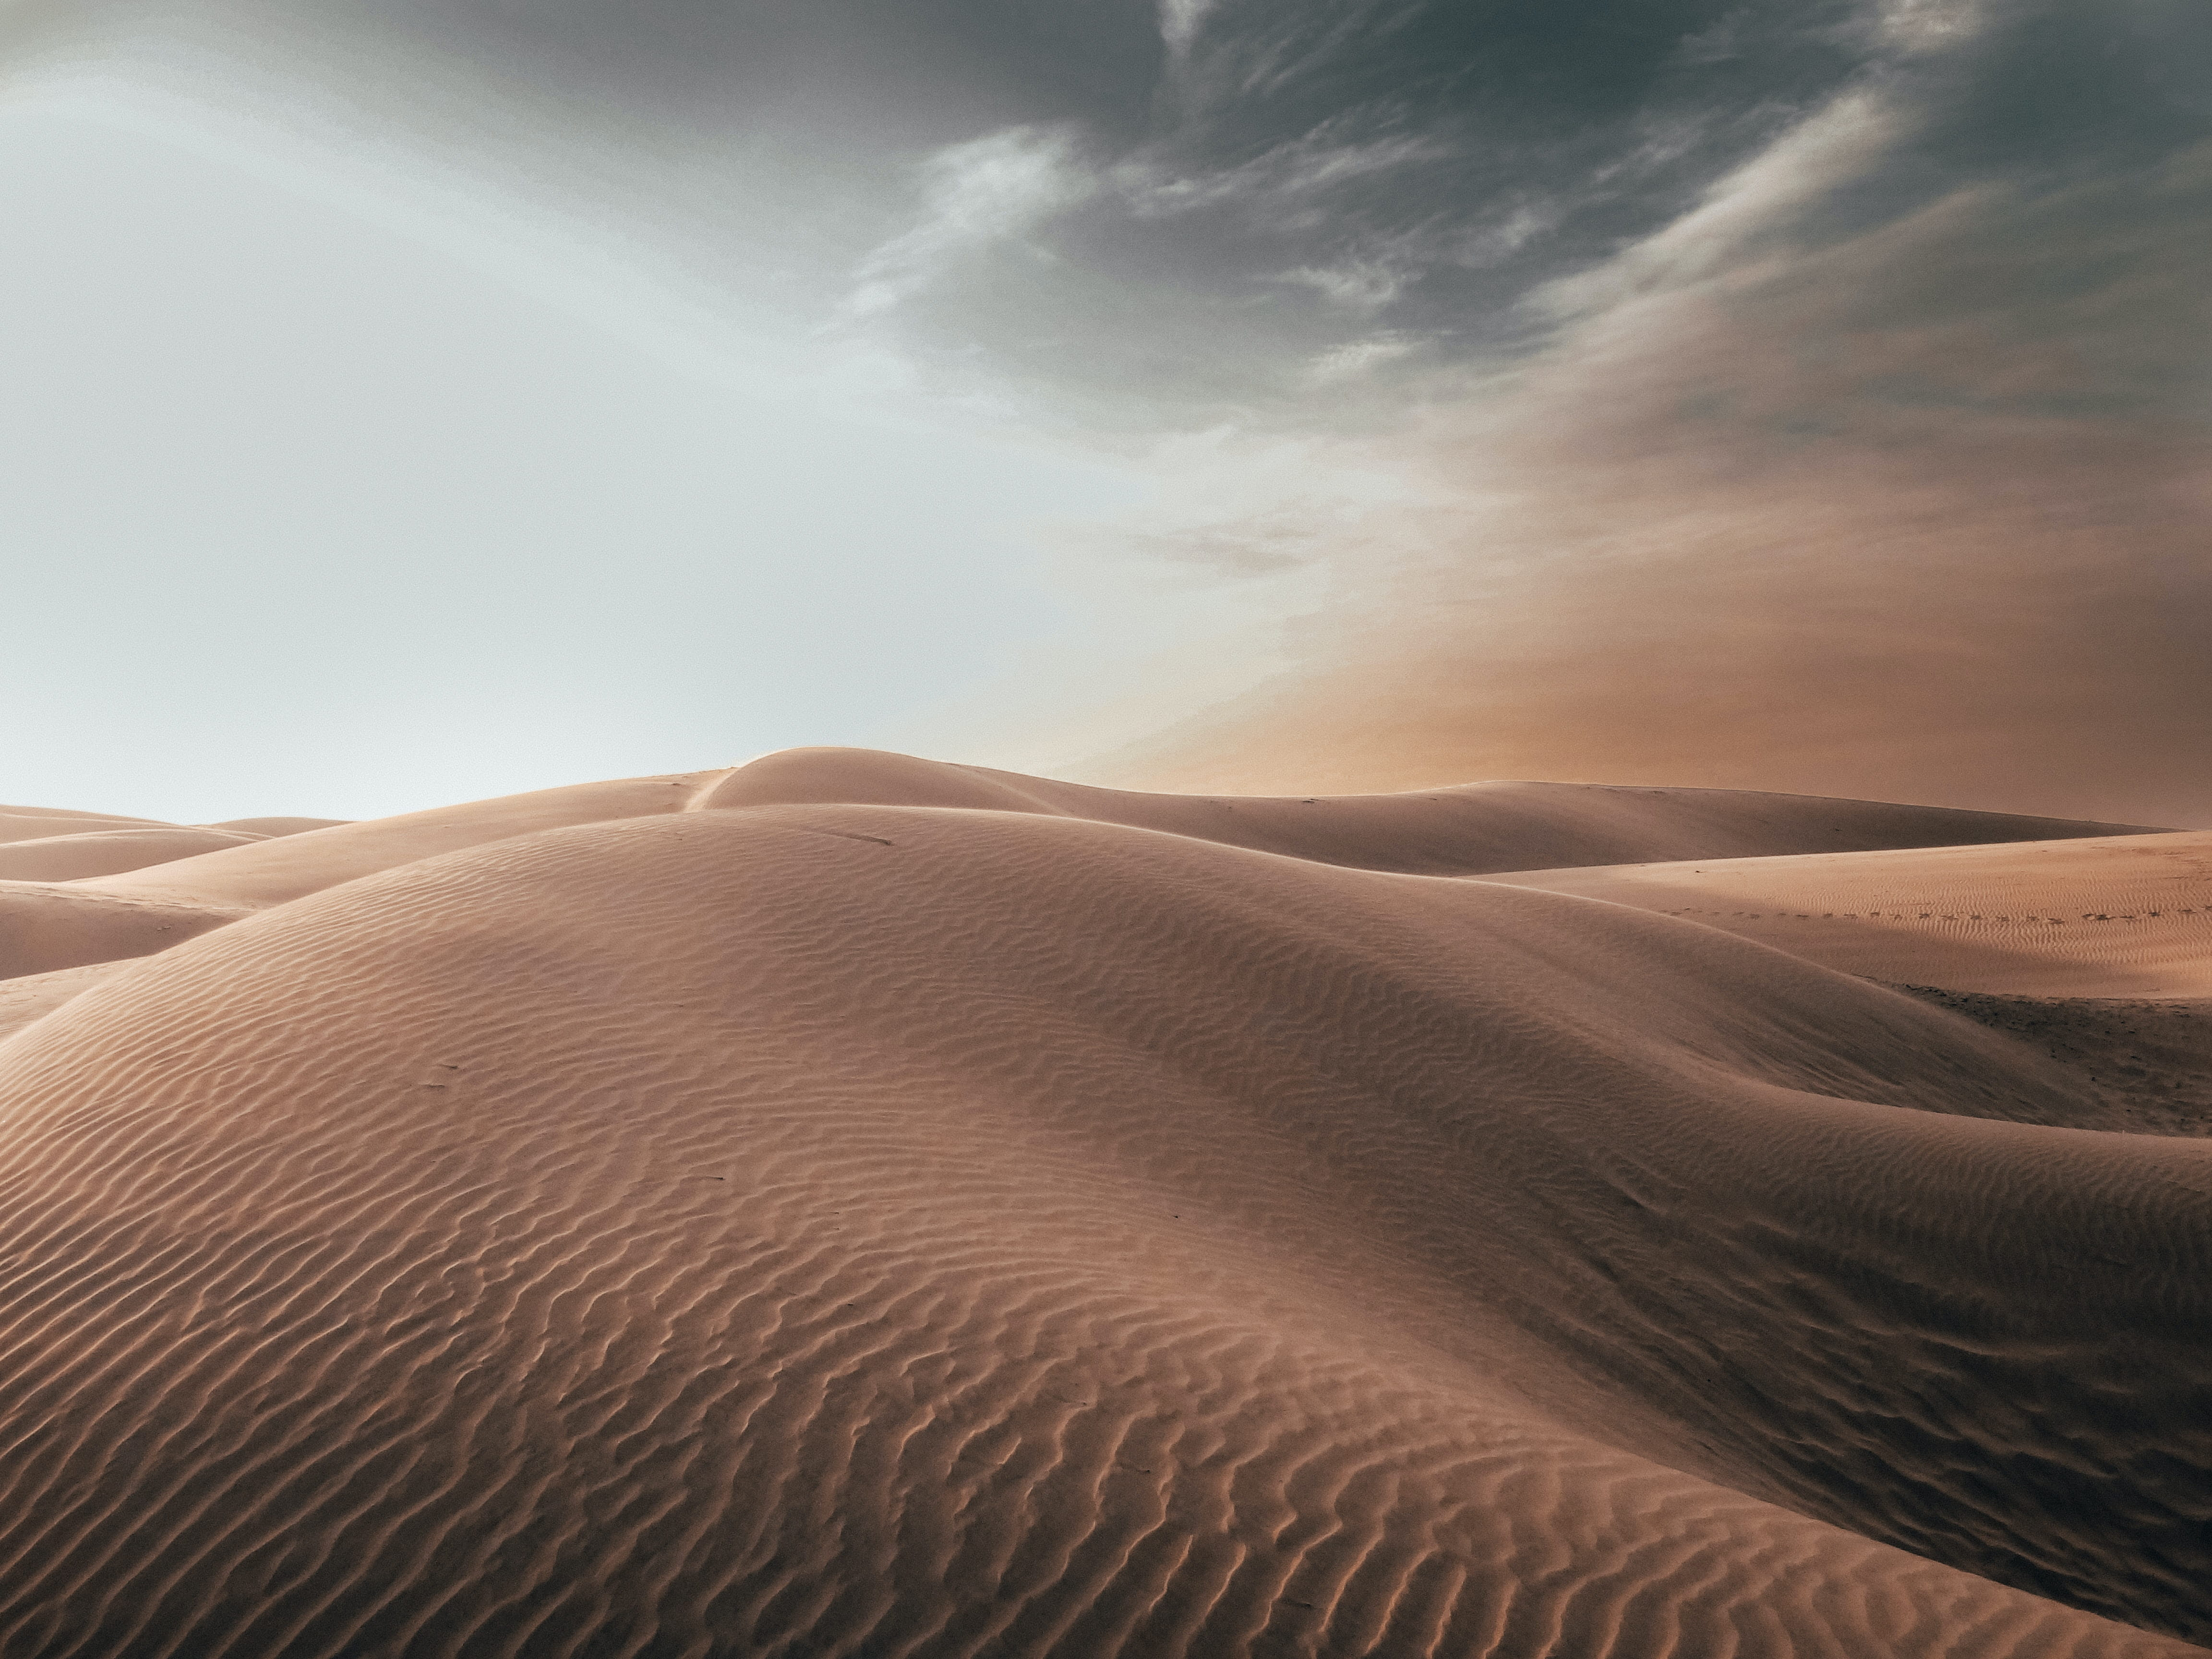
\includegraphics[width=\paperwidth]{duneslides-logo}
}
\begin{frame}[plain,noframenumbering]

	\color{c++reviewduneblue}

	\begin{flushleft}\bfseries\scshape\huge
		Richards model for simulations of water infiltration in
		agricultural soil using DuMu\textsuperscript{x}
	\end{flushleft}

	\

	\

	\

	\

	\

	\begin{minipage}{0.47\textwidth}
		\begin{figure}[ht!]
			\centering
			
\includegraphics[height=2.5cm]{pec3}
			\captionsetup{justification=centering,margin=.2cm}
			\caption*{
				\large
				\bfseries
				\textcolor{c++reviewduneblue}{
					Peruvian Conference on Scientific Computing \\
					October 4, 2022}
			}
		\end{figure}
	\end{minipage}
	\begin{minipage}{0.5\textwidth}
		\begin{flushright}
			\large
			\bfseries
			Made by\\
			John J. Leal Gomez\\
			Guillermo A. Martínez Girón\\
			Arley Martinez Jaramillo\\
			Universidad Nacional de Colombia\\
			Carlos A. Aznarán Laos\\
			Universidad Nacional de Ingeniería, Perú
		\end{flushright}
	\end{minipage}
\end{frame}
}
% 1. Presentación del problema de infiltración de agua
% 1.1 Ventajas de la simulación % Arley ayuda, sin tantas ecuaciones.
% Optimizar el uso del agua en el suelo, lograr el mayor contacto entre las capas periféricas de la raíz del suelo. 1 gota de aceite contamina un litro de agua. riego por surco, problema del percolación, los nutrientes son llevados, ejemplo con el café tradicional. problema
% cantidad desmedida de agua porque el suelo pierde sus nutrientes, %60% de eficiencia
% ejemplo de la caña: pesticidas, exceso de agua, etc (ciclo).
% el perder agua es mucho más caro para la humanidad.
% aportar a la agricultura de precisión
% ruta apoplástica (explica la interacción de la raíz agua)
% % el efecto de las algas (dia/noche) se puede explicar con el cloropasto () y la mitocondria (respiración)
\section{Presentation of water infiltration problem}
% https://i.pinimg.com/originals/34/66/77/34667762422298ffc10fec5252f28619.jpg
\begin{frame}
	\frametitle{\secname}
	\begin{minipage}{0.47\textwidth}
		\begin{figure}[ht!]
			\centering
			\href{https://www.uneditorial.com/las-matematicas-en-la-vida-real-introduccion-basica-el-modelamiento-matematico-matematica.html}{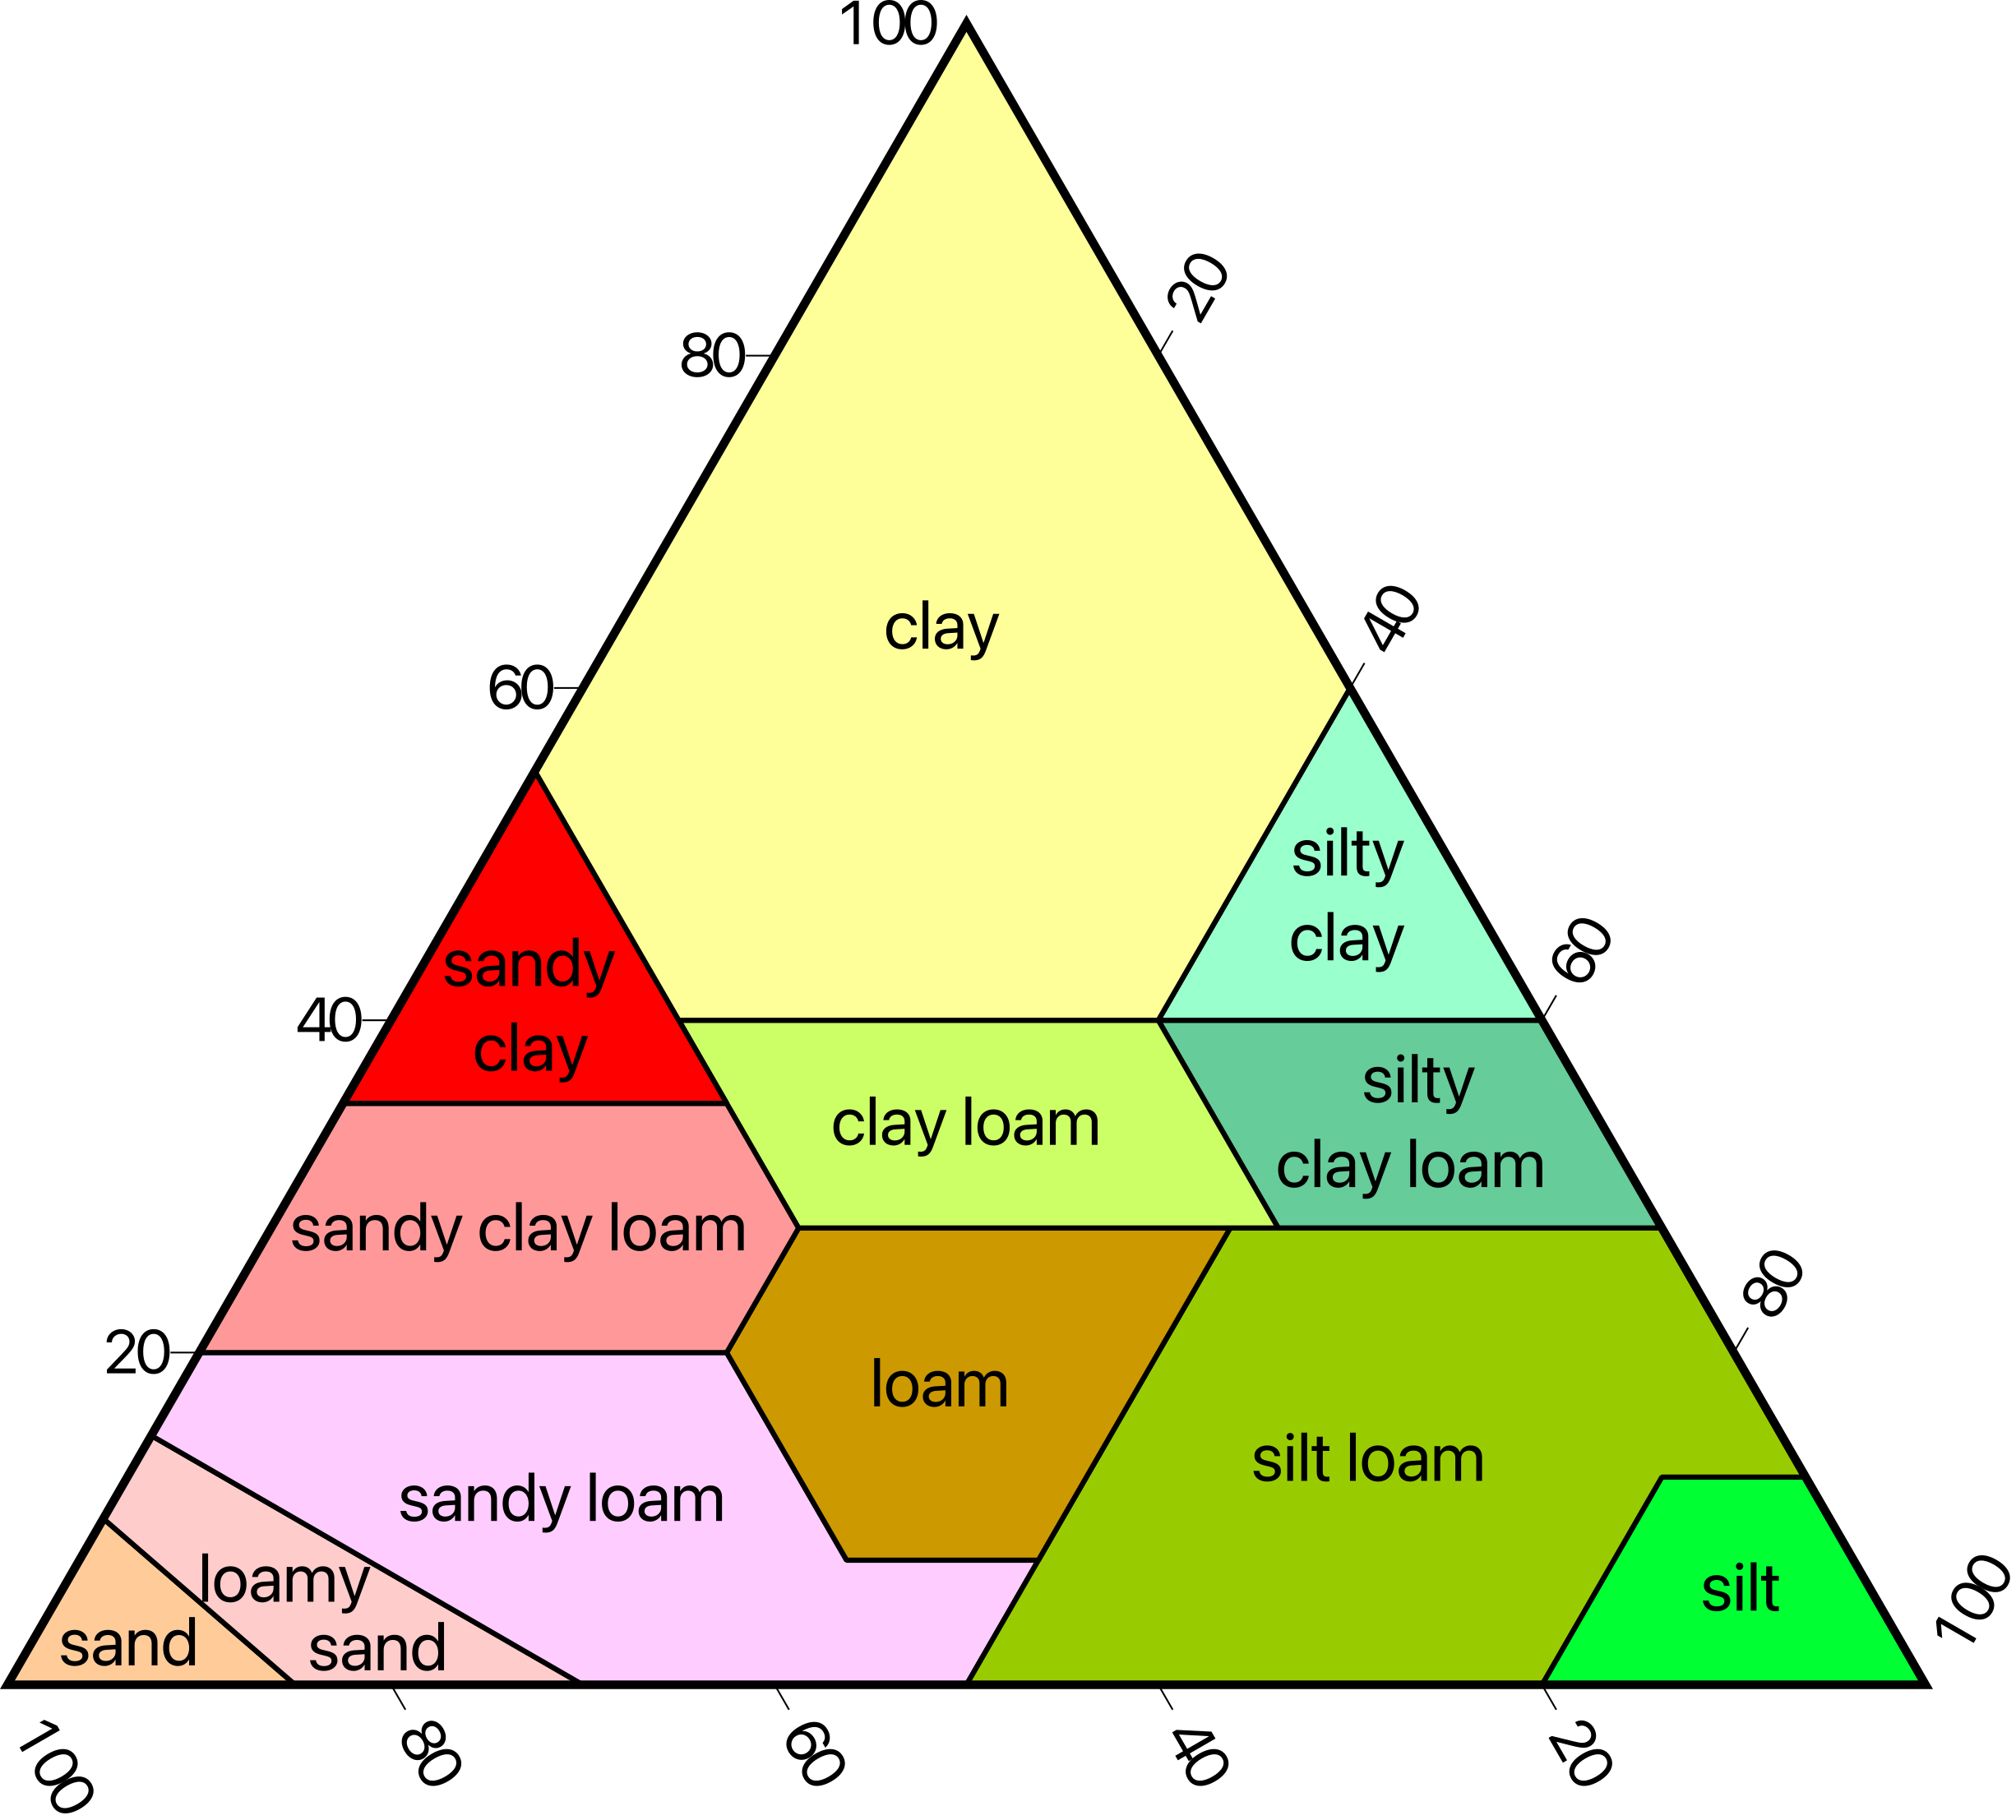
\includegraphics[height=7cm]{textural_soil}}
		\end{figure}
		\note{
			Los autores, John Jairo Leal y Juan Pablo Cardona les compartimos nuestro texto, y les contamos que es el producto de varios proyectos educativos de modelamiento matemático en las aulas en cursos de ingeniería.

			Una de nuestras líneas de investigación es precisamente la educación  matemática para ingeniería y lo que esperamos es que más personas y más profesionales se vinculen con aplicaciones de matemáticas y con desarrollos futuros.
		}
	\end{minipage}
	\begin{minipage}{0.5\textwidth}
		\textsc{\Large Capítulos:}

		\

		\begin{enumerate}
			\item

			      Introducción a los números reales $\mathbb{R}$.

			      \

			\item

			      Introducción a las funciones.

			      \

			\item

			      La derivada.

			      \

			\item

			      Modelamiento matemático.

			      \

			\item

			      Anexos.
		\end{enumerate}
	\end{minipage}
	\note{
		En su estructura el texto es introductorio para los primeros cursos de matemáticas, de hecho lo hemos utilizado en un curso que se llama matemáticas básicas, estudia las funciones y las derivadas y luego muestra algunos ejemplos de la vida cotidiana y cómo éstos se pueden escribir utilizando los símbolos
		matemáticos.
	}
\end{frame}

\begin{frame}
	\frametitle{\secname}
	\begin{figure}[ht!]
		\centering
		\includegraphics[height=7.8cm]{example-image}
	\end{figure}
	\note{
		En la diapositiva se muestra una de estas situaciones diarias.

		También se tiene un anexo donde se estudia un software libre como es \lstinline|wxmaxima|.
	}
\end{frame}
\section{Software simulator for Porous Media Problems}

\begin{frame}
	\frametitle{\secname}

	\begin{alertblock}{DUNE for Multi-\{Phase, Component, Scale, Physics, \ldots\} flow and transport in porous media (DuMu\textsuperscript{x})}
		\note{
			Título: Una introducción a la caja de herramientas DUNE en
			C++/Python para la solución de modelos matemáticos.

			Se hará una breve presentación de la caja de herramientas
			modular Dune Numerics, biblioteca modular desarrollada en la
			Universidad de Heildeberg en C++ y Python, para resolver
			ecuaciones diferenciales parciales utilizando métodos basados
			en mallas, por ejemplo diferencias finitas, elementos finitos o
			volúmenes finitos.

			Es un software de código abierto bajo la licencia GNU General
			Public Licence 2, con binarios disponibles para las
			distribuciones linux Debian, Ubuntu y openSUSE; y
			los scripts de compilación en macOS, FreeBSD, Arch Linux.

			Se mostrará la estructura general, algunos proyectos basados en
			DUNE y algunas simulaciones de modelos matemáticos que incluyen
			éste tipo de ecuaciones y sus respectivas soluciones, así como
			una implementación breve de Dune Numerics.
		}
		\begin{itemize}\small
			\item

			      DuMu\textsuperscript{x} is a multipurpose open-source simulator under the
			      \href{https://www.gnu.org/licenses/lgpl-3.0.html}{
				      GNU Lesser General Public License 3}~\lgpllicense{}.

			\item

			      DUNE is available on
			      \href{https://github.com/dune-copasi/homebrew-tap}{macOS},
			      \href{https://packages.debian.org/search?suite=sid&section=all&arch=any&searchon=sourcenames&keywords=dune-}{Debian}~\debian{},
			      \href{https://launchpad.net/~opm/+archive/ubuntu/ppa}{Ubuntu}~\ubuntu{},
			      \href{https://build.opensuse.org/search?search_text=dune-&search_for=2&name=1&attrib_type_id=}{openSUSE}~\opensuse{},
			      \href{https://aur.archlinux.org/packages/?O=0&SeB=n&K=dune-&outdated=&SB=n&SO=a&PP=50&do_Search=Ir}{Arch Linux}~\archlinux{}
			      and \href{https://www.freshports.org/search.php?stype=name&method=match&query=dune-&num=20&orderby=category&orderbyupdown=asc&search=Search&format=html&branch=head}{FreeBSD}~\freebsd{}.

			      {\fontspec[Renderer=Harfbuzz]{NotoColorEmoji.ttf}🎉}
			      DUNE Release 2.9.0 is planned for end of October 2022.

			\item

			      Porous-Medium Flow, Non-Isothermal, Free Flow, Geomechanics, Pore-Network models.
			      Multidomain, multi-component, multi-phase. Parallel, Grid Adaptivity.

				      {\fontspec[Renderer=Harfbuzz]{NotoColorEmoji.ttf}🎉}
			      Release 3.6.0 is planned for October 7, 2022.

			      \note{
				      Desarrollado con CMake, escrito en C++ con enlaces Python a través de pybind11.

			      }
		\end{itemize}
	\end{alertblock}

	\begin{minipage}{0.45\textwidth}
		\begin{figure}[ht!]
			\centering
			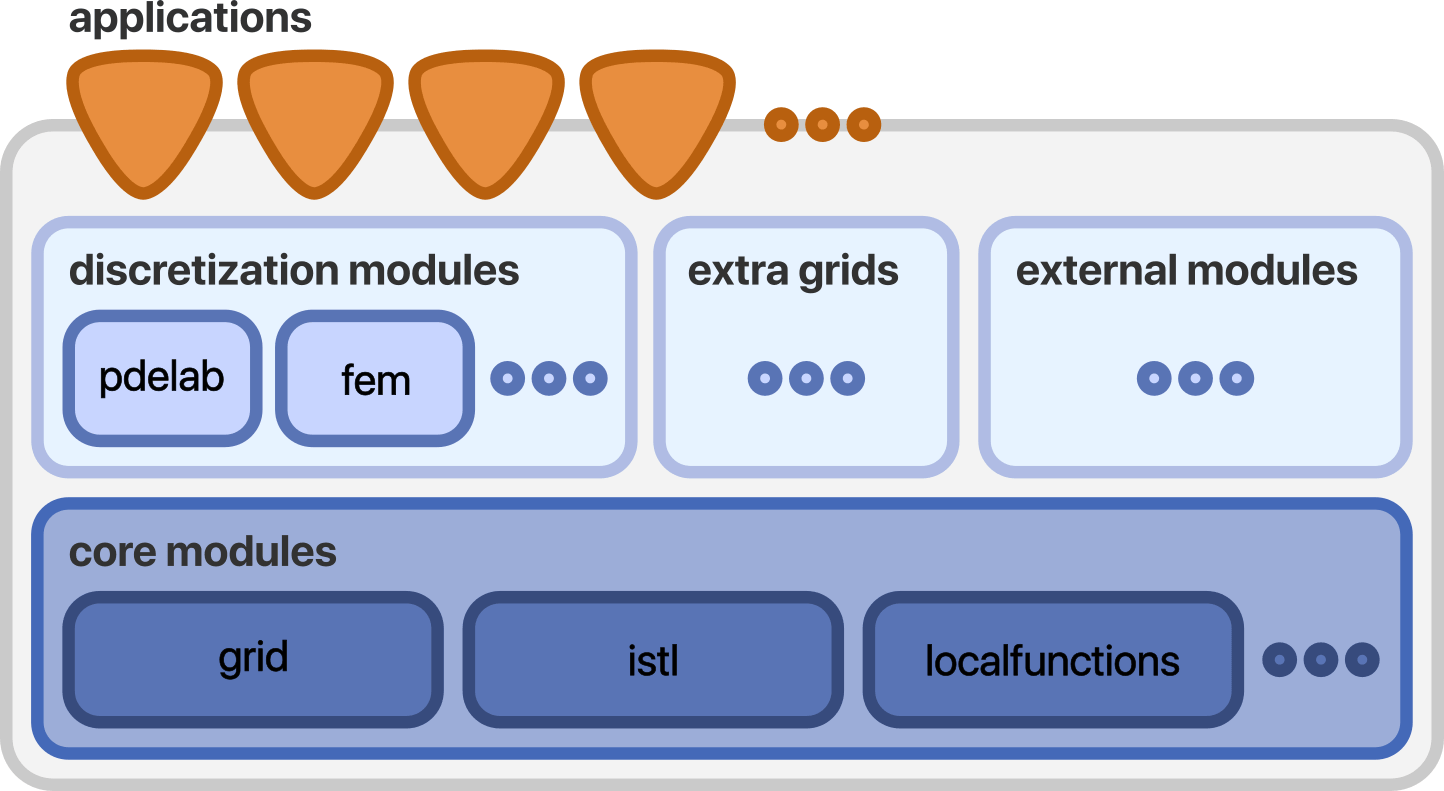
\includegraphics[height=3.2cm]{dunedesign}
			\caption{Taken from \url{https://dune-project.org}.}
		\end{figure}
	\end{minipage}\quad
	\begin{minipage}{0.45\textwidth}
		\begin{figure}[ht!]
			\centering % https://repology.org/project/dumux/versions
			\href{https://github.com/arch4edu/arch4edu}{
\includegraphics[height=2.8cm]{arch4edu}}\quad\quad % dumux simulation picture
			\href{https://github.com/arch4edu/cactus}{
\includegraphics[height=2.8cm]{cactus.png}}
			\caption{Binaries are available in arch4edu repository. (Jingbei Li, Carlos Aznarán, 2022.)}
			% The easiest way to install the binaries are from Arch Linux Repository for Education. Jingbei Li, Carlos Aznarán, et al.
		\end{figure}
	\end{minipage}

\end{frame}

% documentación https://git.iws.uni-stuttgart.de/dumux-repositories/dumux-course
% página principal
% lenguajes
% https://player.vimeo.com/video/572717824
% https://cpp-review-dune.github.io/webinar/slides.pdf
% TODO: Mirar NON-ISOTHERMAL FLUID FLOW RESERVOIR SIMULATION USING DUMUX SOFTWARE
% \input{modules}
\begin{frame}[fragile]
	\frametitle{Snippet en C++}
	\lstinputlisting[caption={Programa \texttt{dune-basics.cc}.},label=dune-basics.cc,]{../../hello_world/test_1p_tpfa.cc}
	\note{
		Se muestra un código minimo de un programa basado en Dune.
		La forma de trabajo es importar las clases con las directivas %\lstinline|#include <dune/modulo/cabecera.hh>|

		\url{https://www.dune-project.org/sphinx/content/sphinx/dune-fem/mcf_nb.html}
		Es una simulación dinámica.
	}
\end{frame}
% \input{archiso}

\begin{frame}\transblindsvertical
	\frametitle{Referencias}
	%------------------------------------------------------------ 1
	\only<1>{
		\begin{itemize}
			\item

			      Books

			      \

			      \nocite{*}
			      \printbibliography[heading=none,keyword=book]
		\end{itemize}
	}

	\

	%------------------------------------------------------------ 2
	\only<2>{
		\begin{itemize}
			\item

			      Articles

			      \

			      \printbibliography[heading=none,keyword=paper]
		\end{itemize}
	}
\end{frame}

\begin{frame}\transblindsvertical
	\frametitle{Referencias}
	%------------------------------------------------------------ 3
	\begin{itemize}
		\item

		      Websites

		      \

		      \printbibliography[heading=none,keyword=online]
	\end{itemize}
\end{frame}
\begin{frame}
	\frametitle{Acknowledgment}
	\begin{center}\Huge
		Thank you so much!
	\end{center}
	\begin{figure}[ht!]
		\centering
		\href{https://www.pec3.org}{
\includegraphics[height=1.7cm]{pec3}}\,
		\href{https://unal.edu.co}{
\includegraphics[height=1.7cm]{unal}}\,
		\href{https://dune-project.org}{
\includegraphics[height=1.5cm]{dune-logo}}\,
		\href{https://dumux.org}{
\includegraphics[height=1.1cm]{dumux}}
	\end{figure}
	\vfill
	\begin{columns}
		\begin{column}{0.5\textwidth}
			\textcolor{c++reviewduneblue!50!c++reviewduneverde}{\href{https://laboratorios.unal.edu.co/geslab2021/servicios-lab-unal/labs-palmira}{\textsc{Laboratorio de Análisis Ambiental}}}

			Sede Palmira, Colombia.

			\

			\textcolor{c++reviewduneblue}{Slides available on:}
			\begin{center}
				\href{https://cpp-review-dune.github.io/flow-test-dumux/slides.pdf}{\url{https://cpp-review-dune.github.io/flow-test-dumux/slides.pdf}}
			\end{center}
			% \textcolor{c++reviewduneblue}{Grabación disponible en:}
			% \begin{center}
			% 	\href{https://player.vimeo.com/video/572717824}{\url{https://player.vimeo.com/video/572717824}}
			% \end{center}
		\end{column}
		\hfill
		\begin{column}{0.5\textwidth}
			\begin{flushright}
				Suggestions or questions to:

				\

				\href{mailto:jlealgom@unal.edu.co}{jlealgom\MVAt unal.edu.co}


				\href{mailto:gumartinezg@unal.edu.co}{gumartinezg\MVAt unal.edu.co}

				\href{mailto:amartinezj@unal.edu.co}{amartinezj\MVAt unal.edu.co}

				\href{mailto:caznaranl@uni.pe}{caznaranl\MVAt uni.pe}
			\end{flushright}
		\end{column}
	\end{columns}

\end{frame}

\end{document}

% 2. La ecuación de Richards
% 2.1. Deducción de la ecuación de Richards (1D o 2D) (Mencionar Darcy)
% 2.1.1 Solución analítica y sus curvas solución con gráficas.
% 2.2.1 Van Genutchen Brookes-Corey model (opcional, pero recomendable)
% 3. El suelo y las características
% 3.1 Parámetros del suelo (triángulo textural) Guillermo, variables físicas
% 3.2 Perfil del suelo, foto de laboratorio de suelos. % Ayuda de Arley, Guillermo.
% 4. Resultados de la simulación % Enlace a la página con el vídeo, un archivo tar.gz
% 4.1. DuMuX (1 hoja)
% 4.1.1 Modelos TFFA, black-box (posiblemente RichardsFOAM)
% 
% Bibliograf'ia

% https://player.vimeo.com/video/572717824
% https://cpp-review-dune.github.io/webinar/slides.pdf (spanish)